\documentclass[30pt]{beamer}
\usepackage{graphicx}
%\usepackage{tikz, flowchart}

%\usetheme{Amsterdam}
\author{ Hsuan-Wei Lee,
  Anzhelika Lyubenko,
  Yuhang Ma,
  Emily Meissen,
  Daniela Velez-Rendon,
    Nara Yoon}


%\vspace{.1truein}

%\begin{center}
%Mentors: John Peach \footnote{Massachusetts Institute of Technology: Lincoln Laboratory}, Cammey Cole Manning\footnote{Mathematics and Computer Science Department, Meredith College},
%Christian Gunning\footnote{Departments of Entomology and Mathematics, North Carolina State University}
%\end{center}
\title[]{Wine, Ebola and Terrorism}

%\date{February 28, 2015}

\begin{document}

\begin{frame}[t,plain]
    \titlepage
\end{frame}

\begin{frame}[t,plain]
    \frametitle{Overview}
\begin{enumerate}
\vfill
\item Introduction
\item Models
\begin{itemize}
\item System-based model
\item Agent-based model
\item Sparial agent-based model
\end{itemize}
\item Comparison
\item Summary
\end{enumerate}
\end{frame}

\begin{frame}
\frametitle{Introduction}
\begin{itemize}
\item Ebola was discovered in 1976
\item 
\end{itemize}
\end{frame}

\begin{frame}
\frametitle{Model}

<<<<<<< HEAD
=======
\begin{figure}[!h]
  \centering
  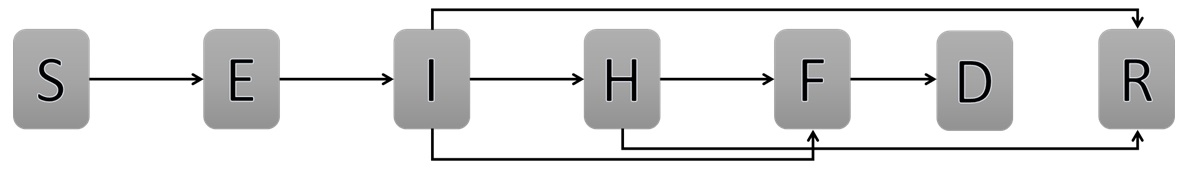
\includegraphics[width=1\textwidth]{compartmentNoFlow}
  \caption{Compartment Model of the Ebola Epidemic in Liberia \newline  Being S: Susceptible, E: Exposed, I: Infectious, H: Hospitalized, F: Funeral,  R: Recovered and D: Dead. } 
\label{fig:compartment} 
\end{figure}
>>>>>>> 39bb738c80778c171147805f700112a1168e22a9
\end{frame}

\begin{frame}
\frametitle{Assumptions}
\end{frame}

\begin{frame}
\frametitle{Parameters/Data}
\begin{figure}[!h]
  \centering
  \includegraphics[width=1\textwidth]{tab_para}
  \caption{Model Parameters for Ebola Epidemic in Liberia Before and After the International Intervention. Calibrated parameters are written in bold font, and posterior means and standard deviations in parenthesis are notated. } 
\label{fig:compartment} 
\end{figure}
\end{frame}

\begin{frame}
\frametitle{Parameters/Data}
\begin{figure}[!h]
  \centering
  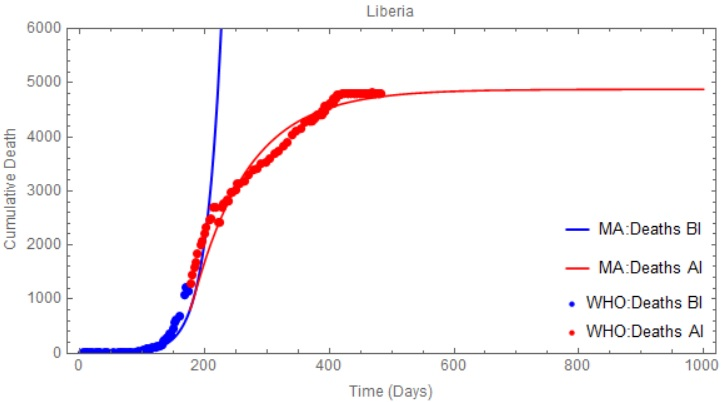
\includegraphics[width=1\textwidth]{CumulativeDeathMathematica}
  \caption{Validation of calibration. Dots represent cumulative death data and the lines represent simulation
based on mean posterior parameters. (Blue) - pre intervention and (red) - post treatment.} 
\end{figure}
\end{frame}


\begin{frame}
\frametitle{System model}
\end{frame}

\begin{frame}
\frametitle{System Model Results}
\begin{figure}[!h]
  \centering
  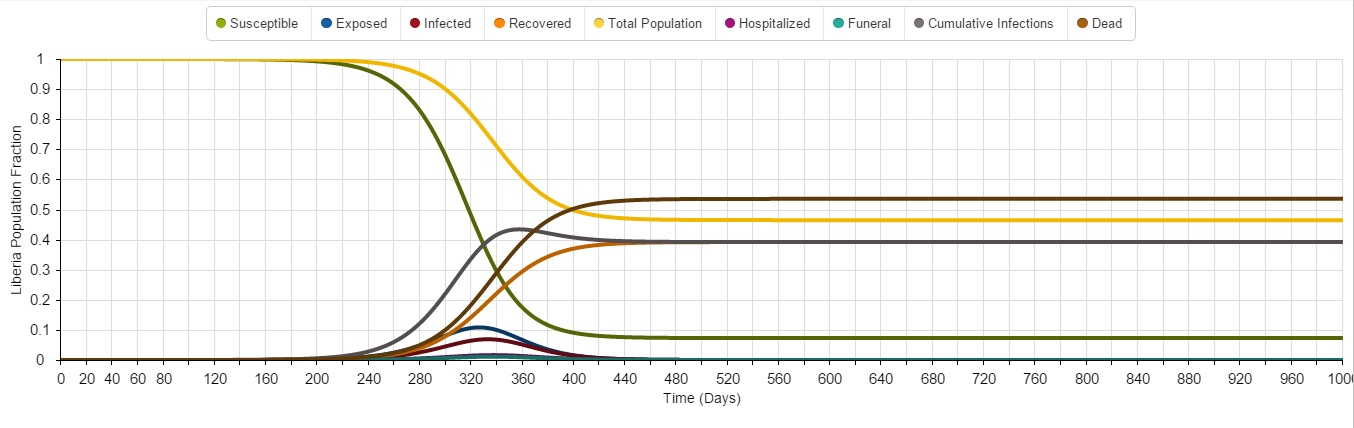
\includegraphics[width=1\textwidth]{LB_NoInt_SD_IM}
  \caption{ Insight Maker results using the parameters of the first stage (Mar/14 to Sept/14) and assuming no intervention}
\label{fig:LB_IM_NoIn} 
\end{figure}
\end{frame}

\begin{frame}
\frametitle{System Model Results}
\begin{figure}[!h]
  \centering
  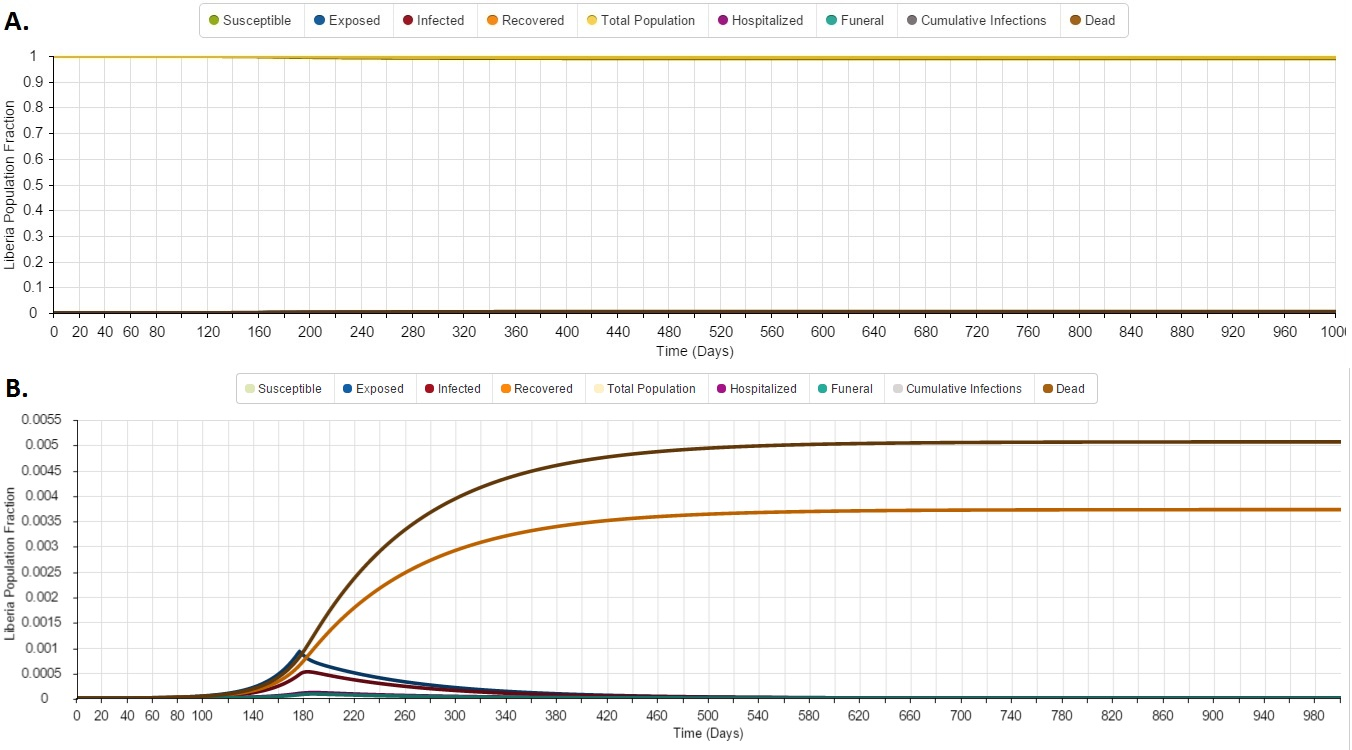
\includegraphics[width=1\textwidth]{LB_Int3_SD_IM}
  \caption{ Insight Maker results. \textit{Top:} parameters of the first stage (Mar/14 to Sept/14), \textit{Bottom:} parameters of the second stage ( Sept/14 to July/15)}
\label{fig:LB_IM_In} 
\end{figure}
\end{frame}

\begin{frame}
\frametitle{System Model Results}
\begin{figure}[!h]
  \centering
  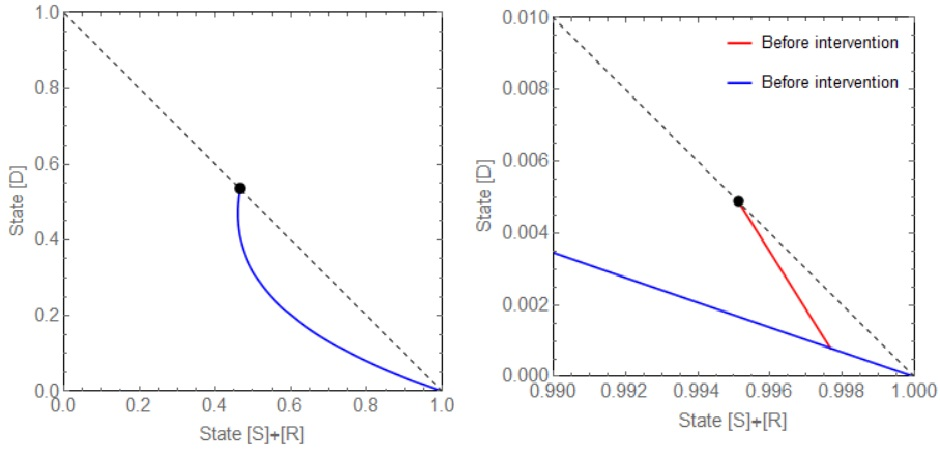
\includegraphics[width=1\textwidth]{PhasePortrait}
  \caption{ Projection of phase portrait to (Susceptible + Recovered, Dead) space. (Blue) - without intervention,
(Red) - with intervention, (Dots) - where the phase converges (equilibrium).}

\end{figure}
\end{frame}




\begin{frame}
\frametitle{Agent model}
MAYBE INCLUDE DIAGRAM
\begin{itemize}
\item Probabilistic model vs. deterministic
\item Flows become probabilities
\item Individuals vs. system
\begin{itemize}
\item 1000 individuals; 1 exsposed
\item 500 days
\item 100 repetitions
\end{itemize}
\end{itemize}
%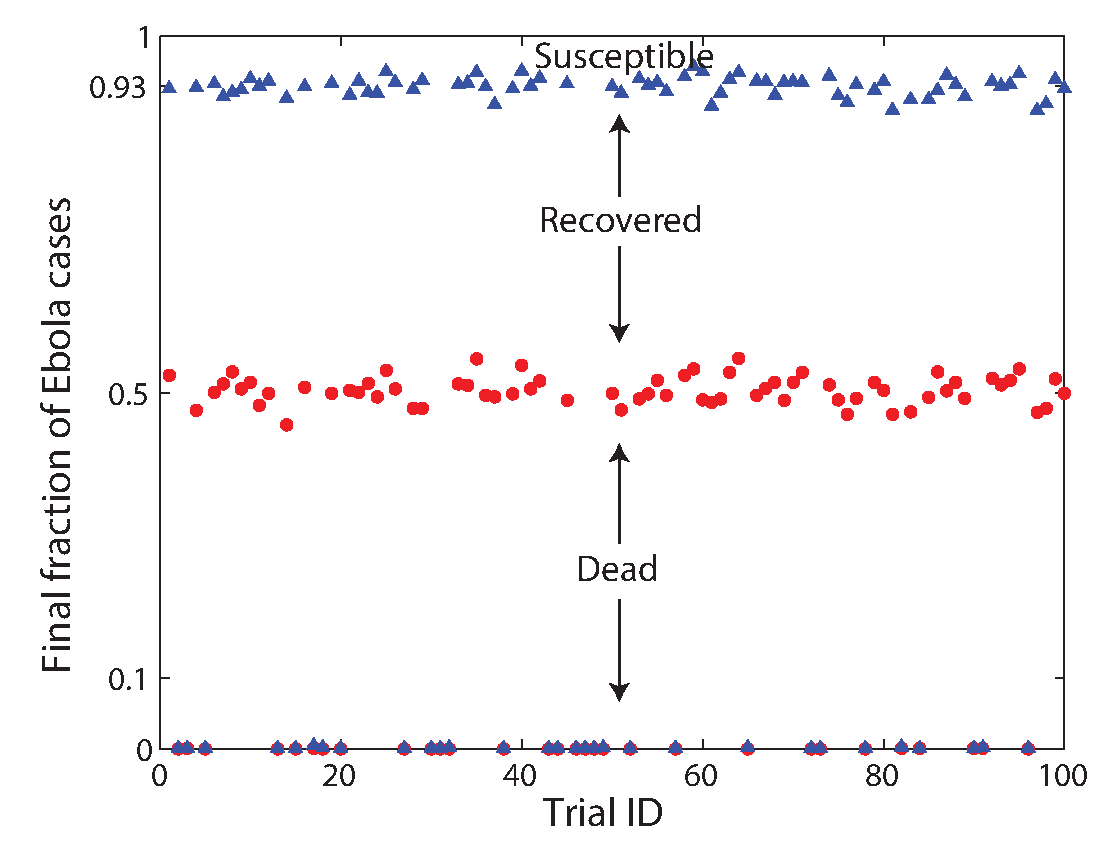
\includegraphics[scale=0.5]{N1000Scatter.eps}
\end{frame}

\begin{frame}
\frametitle{Agent Model Results}
30 PERCENT OF THE TIME WE DO NOT GET AN OUTBREAK BUT WHEN WE DO CONSEQUENCES ARE SEVIER; A TYPICAL OUTBREAK LOOKS AS FOLLOWS
\textbf{Timeseries Plot}
\textbf{Histogram number of cases as a function of number of infected}
\end{frame}

\begin{frame}
\frametitle{Spatial Agent Model}
\end{frame}


\begin{frame}
\frametitle{Spatial Agent Model Results}
\end{frame}

\begin{frame}
\frametitle{Comparison}
\end{frame}

\begin{frame}
\frametitle{Summary}
\end{frame}
\end{document}